%
    \bigskip%
    The fundamental plasma physics needed for this thesis has now been introduced. Further details can be found in~\cite{Piel10,Schulze09,Meichsner13}. To get an insight into the microscopic processes in a ccrf discharge I will use a kinetic Particle-in-Cell simulation. A kinetic model is needed to be able to resolve the distribution functions properly, which is required to be able to answer my second research question, namely the influence of surface effects on the distribution functions of negatively charged oxygen ions measured at the grounded electrode. Low pressure, low temperature radio frequency discharges are non-thermal plasmas with long mean free paths. Therefore,  energy/velocity distribution functions are not Maxwellian and fluid models fail. A kinetic PIC code with Monte-Carlo-Collisions is used, which is introduced here.%
    \bigskip
%
	\section[Particle-in-Cell Simulations including Monte Carlo-Collisions]%
	        {Particle-in-Cell Simulations including%
	        \\Monte-Carlo-Collisions}\label{sec:picsimulationmcc}
%
	Particle-In-Cell simulations including Monte-Carlo-Collisions (PIC-MCC) represent a powerful tool for fully kinetic plasma studies. They provide a self-consistent solution, including reaction and collision routines. They are used in all branches of plasma physics, ranging from simple laboratory discharges to electric propulsion devices, fusion plasmas and interplanetary astrophysical systems. 
	A PIC algorithm simulates the motion of pseudo-particles in a continuous phase-space. Macro-quantities like forces, fields and densities are stored and calculated on a grid. The number of calculations needed per step to solve the equation of motion for each of the $N$ particles sums up to $N\log(N)$, in contrast to particle-particle codes which a scale like $N^2$. The self-consistent electrostatic macro-fields are calculated by solving \emph{Poisson's equation}.\\
	In the following the basic scheme of a PIC-MCC simulation will be explained. As it was outlined by~\autoref{sec:chapter_ccrfbasics}, I will focus on the electrostatic case with $\vec{B}=0$, as the magnetic field generated from the moving charged particles is small enough that the Lorentz force is dominated by the electric field $q\ix{j}\vec{E}$.
%	
		\subsection{Principles}\label{sec:picbasics}
%
			\begin{figure}[!b]
				\centering
				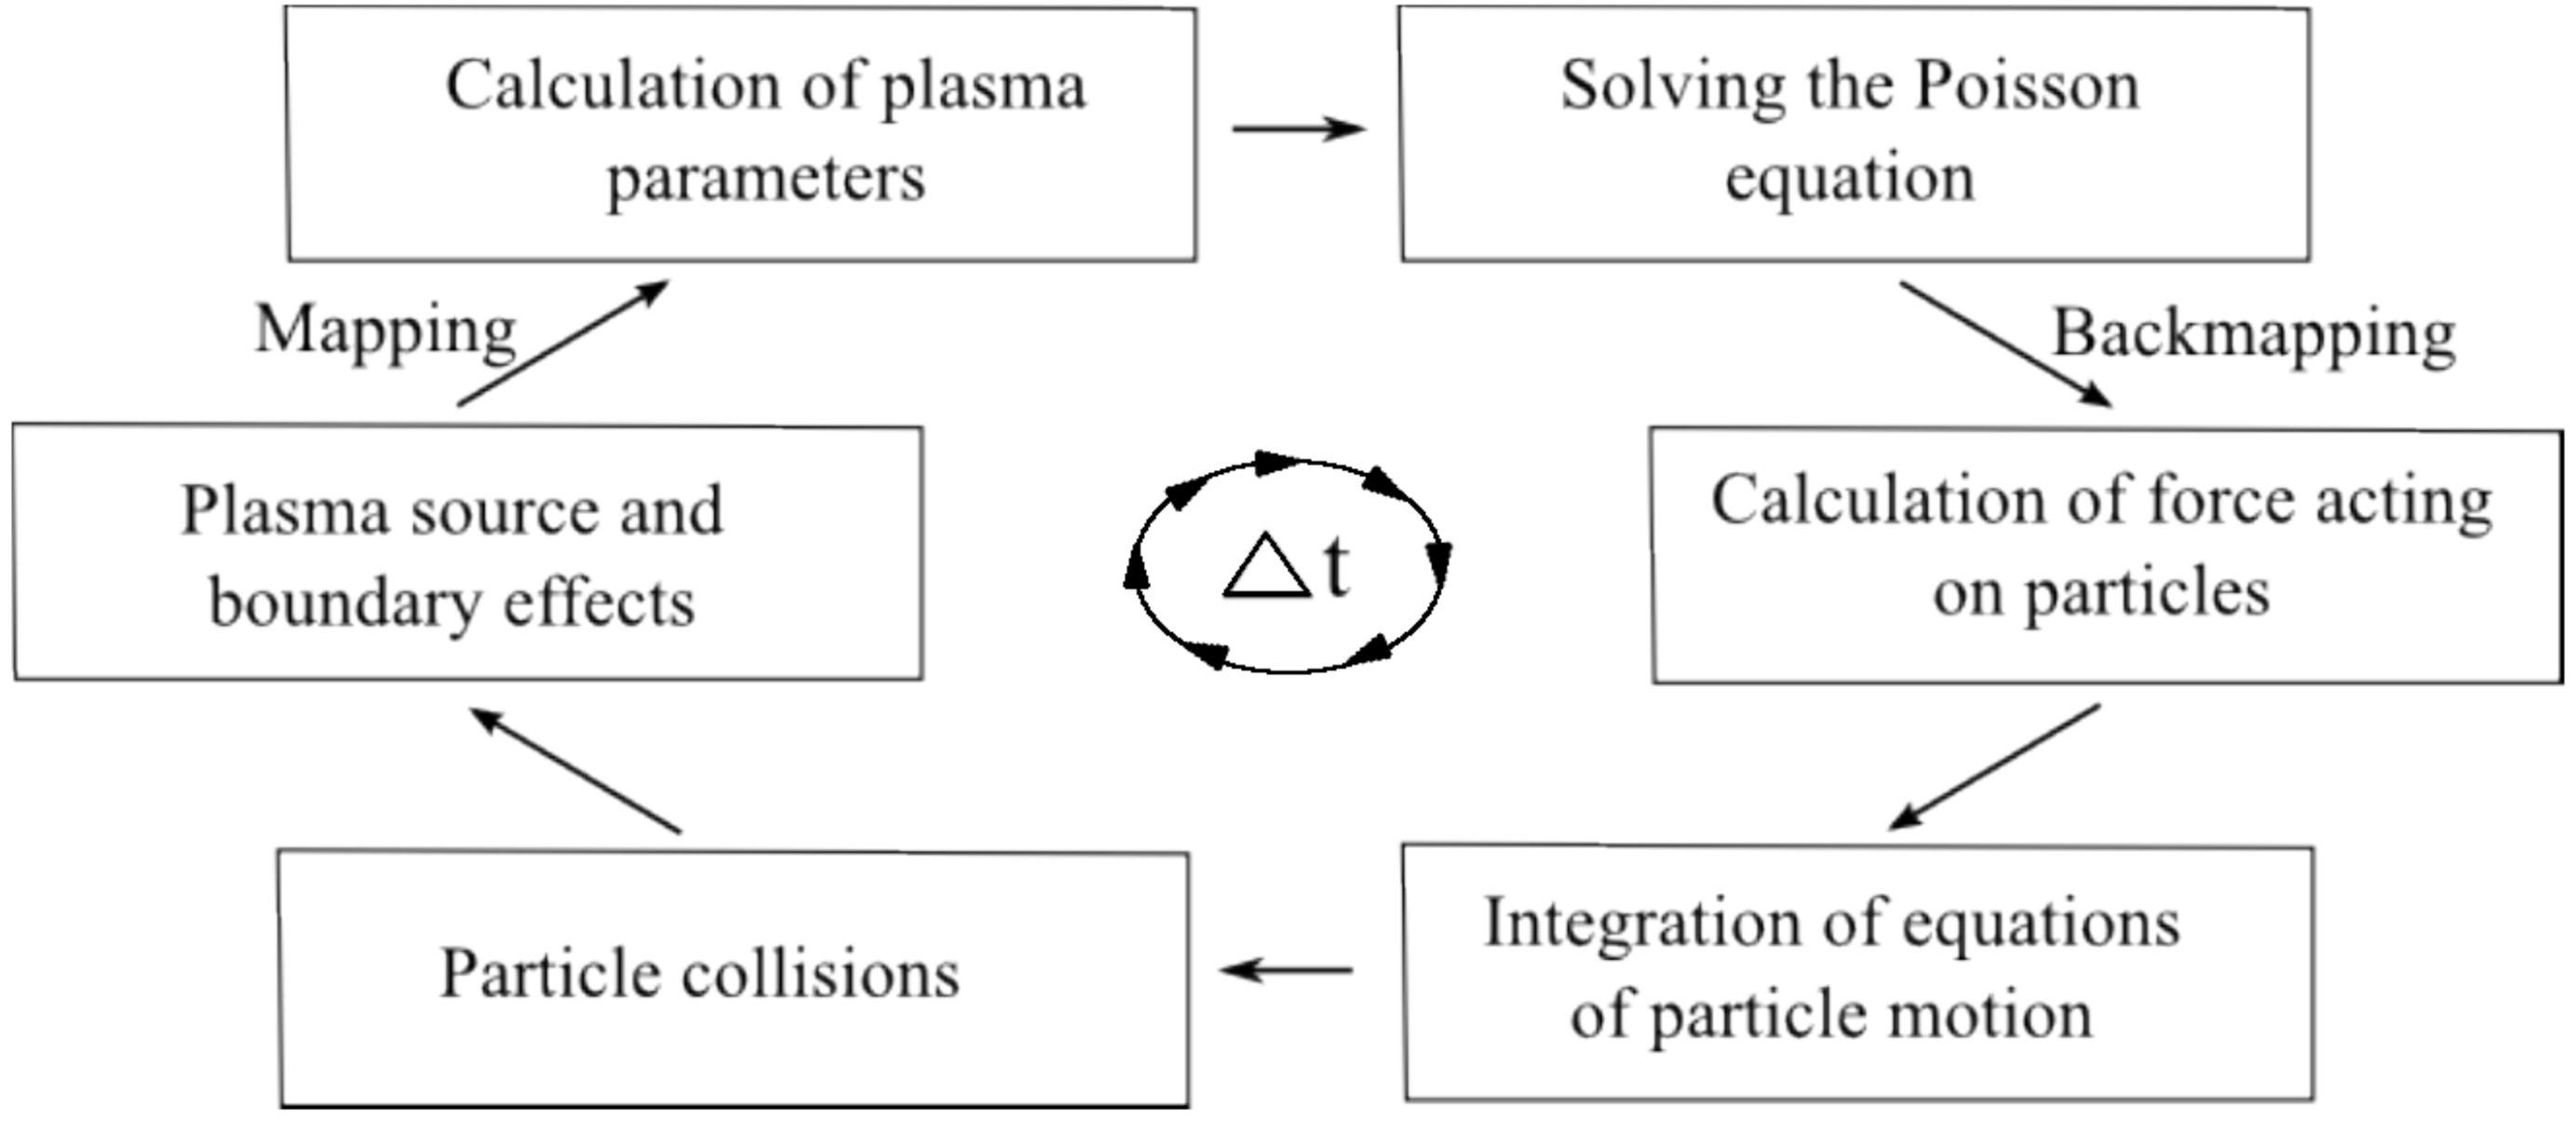
\includegraphics[width=1.0\textwidth]{figures/picscheme.pdf}
				\caption[PIC simulation scheme]{%
				PIC simulation scheme~\cite{Matthias15}.}\label{fig:picscheme}
			\end{figure}
%			
		In general, the spatio-temporal evolution of the velocity distribution function $f\ix{j}(\vec{v},\vec{r},t)$ is given by the \emph{Boltzmann equation}:
%
			\begin{align}
				\frac{\partial f\ix{j}}{\partial t}+\vec{v}\cdot\nabla_{\vec{r}}\,f\ix{j}%
					+\frac{q\ix{j}}{m\ix{j}}\vec{E}\cdot\nabla_{\vec{v}}\,f\ix{j}%
					=\left(\frac{\partial f\ix{j}}{\partial t}\right)\ix{Coll}\,.%
				\label{equ:boltzmannequation}
			\end{align}
%
			In this equation, the product of $q\ix{j}\vec{E}/m\ix{j}$ denotes the electrostatic force onto the particle of species $j$. The velocity and space gradient are calculated like $\nabla_{\vec{r}}\,f\ix{j}=\partial f\ix{j}/\partial x\cdot\vec{e}\ix{x}+\dots$ and so on. The right hand side of $(\partial f\ix{j}/\partial t)\ix{Coll}$ is the sum of all collision effects on $f\ix{j}(\vec{v},\vec{r},t)$. One approach would be an integral form, in which all probabilities of a two-body interactions with different incident and outgoing velocities are summed up in a convolution integral with $f\ix{j}(\vec{v},\vec{r},t)$.\\
			The approach via the distribution function yields the advantage of an easy access to the afore-mentioned macro-quantities, the zeroth and first moment are noted below in~\autoref{equ:zeorthandfirstmoment}. Using the moments, one can write down $f\ix{j}(\vec{v},\vec{r},t)$ at a thermodynamic equilibrium of $T\ix{j,0}$ as the \emph{Maxwell-Boltzmann-distribution-function} like so:
%
			\begin{align}
				n\ix{j}(\vec{r},t)=q\ix{j}\int_{-\infty}^{\infty}%
					f\ix{j}(\vec{v},\vec{r},t)\diff\vec{v}\,,%
					\quad\quad%
					\langle v\ix{j}(\vec{r},t)\rangle=\frac{1}{n\ix{j}(\vec{r},t)}%
					\int_{-\infty}^{\infty}\vec{v}f\ix{j}(\vec{v},\vec{r},t)\diff\vec{v}%
				\label{equ:zeorthandfirstmoment}\\[0.3cm]
				f\ix{j}(\vec{v},\vec{r},t)=\frac{n\ix{j}(\vec{r},t)}%
				    {q\ix{j}}\,\hat{f}\ix{j}(\vec{v},\vec{r},t)%
					=\frac{n\ix{j}(\vec{r},t)}{q\ix{j}}\,{\left(\frac{m\ix{j}}%
					{2\pi k\ix{B}T\ix{j,0}}\right)}^{3/2}%
					\,\exp\left(-\frac{|\vec{v}\ix{j}|^{2}}{v\ix{j,th}^{2}}\right)%
				\label{equ:maxwellboltzmannfunction}
			\end{align}
%
			In a Maxwellian plasma one could use a fluid approach, where the moment equations for all species are solved. This would reduce the computational cost drastically, as one would no longer have to track each particle individually, and sufficiently describe the discharge by charaterisation of macro-quantities. This is valid, if mean-free-paths are small and collisions rather likely, producing a Maxwellian distribution function. However, in a low-temperature, low-pressure ccrf discharge mean-free-paths are large and collisions are rare, which is why a fully kinetic Particle-in-Cell simulation method is used.\\
			For a N-particle system $n$-th equation of motion in the $N$-particle system becomes:
%
			\begin{align}
				\frac{\diff \vec{x}\ix{n}}{\diff t}=\vec{v}\ix{n}\,,%
					\quad\quad\quad%
					\frac{\diff \vec{v}\ix{n}}{\diff t}=\frac{1}{m\ix{n}}%
					\vec{F}\ix{n,L}(\vec{x}\ix{n},\vec{E},t)%
					=\frac{q\ix{n}}{m\ix{n}}\vec{E}(\vec{x}\ix{n},t)%
				\label{equ:equationofmontionpic}
			\end{align}
%
			where $F\ix{n,L}$ is the \emph{electrostatic Lorentz force}.\\
			The number of $N$ is of orders of magnitude higher than what the best supercomputers can handle. Hence it is assumed that one simulated particle at $\vec{x}\ix{n}$ and velocity $\vec{v}\ix{n}$ represents many physical particles. This \emph{super-particle factor} is usually between $\tenpo{3}$--$\tenpo{4}$, depending on the size and initial density in the simulated domain. Those super-particles follow the same dynamic and kinetic behaviour like their physical counterparts, because they have the same charge to mass ratio. By this, also mathematically proven, a correct solution of the kinetic equation is guaranteed.\\
			To solve for the electrostatic force $F\ix{n,L}$, the total charge density has to be calculated by interpolating the point charges $q\ix{n}$ of each particle onto the point grid (\autoref{equ:interpolation}). The Interpolation of particle densities to mesh points and back-mapping of the electric field to particle positions have to use the same interpolation function (usually linear) to guarantee momentum conservation.\\
			Poisson's equation is solved globally by using the interpolated charge density on that grid (\autoref{equ:poissonpotential}). This gives the the electric field:
%
			\begin{align}
				\rho(\vec{r},t)&=\rho(\vec{x}\ix{1},\vec{x}\ix{2},\dots,\vec{x}\ix{N},t)\,,%
					\label{equ:interpolation}\\[0.0cm]
				\Rightarrow%
				\Delta\Phi(\vec{r},t)&=-\frac{\rho(\vec{r},t)}{\varepsilon\ix{0}}\,,%
					\label{equ:poissonpotential}\\[0.0cm]%
					\Rightarrow\hspace*{7pt}%
				\vec{E}(\vec{r},t)&=-\nabla\Phi(\vec{r},t)\,.%
					\label{equ:efieldmaxwell}
			\end{align}
%           
            A standard approach to obtain the solution of Poisson's equation is the \emph{finite-difference method}. For a two-dimensional, with $\Delta r$ equally partitioned mesh at ($r^{(1)}\ix{l}$,$r^{(2)}\ix{m}$) one yields the \emph{five point stencil}:
%
		\begin{align}
			4\Phi\ix{l,m}-\Phi\ix{l-1,m}-\Phi\ix{l+1,m}-\Phi\ix{l,m-1}-%
				\Phi\ix{l,m+1}=\Delta r^{2}\cdot\frac{\rho\ix{l,m}}{\varepsilon\ix{0}}%
				\label{equ:fivepointstar}
		\end{align}
%
        The discrete matrix~\autoref{equ:poissonpotential} is solved using a \emph{LU-factorisation}. On the system side this process is optimised by the matrix-solver library~\emph{SuperLU} for the direct solution of large, sparse non-symmetric systems of linear equations. There exist also other matrix-solver algorithms, for example the successive-over-relaxation (SOR) or gradient descent method.\\
		The potential is calculated on every time step using this factorisation, but the latter is done only once at the beginning, because it only depends on the mesh, and hence the composition of the matrix $\Phi\in\mathbb{R}^{N\ix{r}\times N\ix{z}}$. At this is point any potential boundary conditions, such as external voltages $U\ix{rf}(t)$ or ground $\Phi=0$ are applied to the result of $\Phi$.\\
		In our simulation, the dimension of time is also represented by a grid. The stepping is done for a constant width $\Delta t$: $t\rightarrow t\ix{k}=t\ix{0}+k\, \Delta t$ (and correspondingly all other physical properties).	Integrating the equations of motion at a given time step $t\ix{k}$ from~\autoref{equ:equationofmontionpic} is done by an energy conserving integrator scheme called Boris algorithm. It is used to calculate the new velocities and positions. To move the particle of index $n$ and species $j$ the following equations have to be solved at the time step $k$, or $k+/-\frac{1}{2}$ respectively (leap frog scheme):
%
			\begin{align}
				\vec{u}\ix{n,+}=\vec{v}\ix{n,k-1/2}+h\cdot\vec{E}\ix{k}\,,%
					\quad\quad%
					h=\frac{q\ix{j}}{2\,m\ix{j}}%
					\nonumber
				\end{align}\vspace*{-0.8cm}\begin{align}
				\boxed{%
					\vec{x}\ix{n,k+1}=\vec{x}\ix{n,k}+\Delta t\vec{v}\ix{n,k+1/2}%
						\quad\text{~and~}\quad%
						\vec{v}\ix{n,k-1/2}=\vec{u}\ix{n,+}+h\cdot\vec{E}\ix{k}\, ,%
						\label{equ:leapfrogscheme}%
					}
			\end{align}
%			
			Spatial and temporal step width are crucial to the results and performance of the simulation. Due to the coupling of particle and mesh methods in the PIC algorithm, certain requirements for numerical stability have to be satisfied for the mesh size $\Delta r$ and time step $\Delta t$ by
%
		\begin{align}
			\boxed{%
				\Delta t\ix{0} \le \SI{0.2}\cdot\omega\ix{p,e}%
					\quad\text{~and~}\quad%
					\Delta r\ix{0} \le \SI{0.5}\cdot\lambda\ix{D,e}\,.%
					\label{equ:stabilitycriteria}%
				}
			\end{align}
%
			The spatial and temporal step width should sufficiently resolve the smallest and fastest processes in the simulated model. Hence the physical scales of electron plasma frequency $\omega\ix{p,e}$ and electron Debye length $\lambda\ix{D,e}$ are chosen. In the PIC simulation they are used in a dimensionless form. Every other property is written the same way in relation to the electron plasma frequency and Debye length. Thus the complete algorithm becomes dimensionless. Electron bulk density and temperature are estimates for the necessary spatio-temporal resolution of the plasma and the simulated discharge equilibrates self-consistently. Therefore one has to check the results for under- or over-resolution. If the spatial partitions are made too small, e.g.\@ the bulk density is much smaller than the estimated value, the necessary computation time rises. If vice versa non-physical behaviour might be observed in the simulation.\\
			We will only consider the movement of charged species during the simulation. Transport of neutrals is neglected in this work, because the distribution of the neutral gas reservoir can be considered homogeneous due to their very large mean free path of 2-$\unit[30]{cm}$, depending on the pressure. Also, because the neutral species is cold and has a very slow drift velocity --- and therefore a large time scale of the transport process in the range of a couple $\unit{ms}$ --- the O$\ix{2}$ are implemented as a stationary, inexhaustible reservoir at a constant density/pressure and temperature of $T=\,$\SI{300}{\kelvin}. Though collision routines are still exercised, and the neutral particles do have velocity components differing from zero, the corresponding movement of the neutral species is not calculated.\\
			Additionally an amplification factor is calculated to account for the real density of physical neutral gas particles. This is only used when collision probabilities are calculated, so that the processes with $O^{2}$ are not under-represented. It is usually between \SIrange{1e7}{1e8}, depending on the pressure.\\
			Because we know that the electrons are the fastest species in the discharge, and the time step is chosen to sufficiently describe all plasma processes, one can significantly save computation time when pushing the slower species less often. Therefore a subcycling routine is used, which pushes the heavier and slower ions only every few steps, e.g\@ 2-6 code cycles. The subcycling factor is sensitive to the species velocities, because the particles should not be pushed further than one Debye length $\lambda\ix{D}$ to avoid numerical problems. The subcycling method is also applied to the collision routine, which again saves more computational time. Forces acting upon the slower particles have to be summed up and average in the mean time.\\
			After all the particles of index $n$ are pushed according to the calculated velocity $v\ix{n,k+1/2}$ and previous position $x\ix{n,k}$ to their new position $x\ix{n,k+1}$, boundary conditions such as secondary emission, reflection and absorption at walls are applied. Those processes are in general far from trivial. Therefore, a \emph{Monte-Carlo} algorithm is used, in which a random generated number $R\in[0,1]$ is compared with the probability $P(\theta,E)$ of a corresponding physical process, e.g.\@ secondary emission. This probability is a function of incident angle $\theta$ and energy $E$. For $P>R$ the secondary particle of species $j$ is injected with a given velocity distribution $f\ix{j}^{sec}(\vec{v})$, other wise the projectile is just lost (see~\autoref{sec:surfaceeffects} and~\autoref{sec:negionphysics}).\\
			To summarise this section, a basic simulation code cycle for one time step of a PIC-MCC method is shown in~\autoref{fig:picscheme}. More details can be found in~\cite{Tskhakaya}.
%
            \par%
            After the PIC method has been outlined one will highlight the used collision routines and corresponding reaction set of oxygen. The importance of collisions in ccrf discharges has been discussed before in e.g.\@~\cite{Surendra93,Bronold07b,Gudmundsson13}. Furthermore, the selection of reaction sets and collisional routines respectively have been firstly proposed by Matyash~\cite{MatyashDiss} for this PIC simulations. There a more in-depth approach can be found.\\
            Because I want to investigate the negative ion dynamics, the plasma chemistry and corresponding collisions need to be discussed here. In the following paragraph and sections I will sketch the collisions and algorithms used in the PIC simulation. Therefore, an anion reaction set is firstly introduced to the two-dimensioanl PIC code.%
            \par%
%            
		\subsection{Collision Routines}
%		
			 In contrast to a global method, which calculates every single of the $N^{2}$ particle-particle interactions, a binary collision model is used for coulomb collisions. In this algorithm only particles from the same Debye cell are considered to collide with each other. Because self-forces where excluded from the simulation by the weighting scheme in the previous section, the inter-particle forces inside grid cells are underestimated. This can partially be compensated when introducing the binary collision operator. This still satisfies energy and momentum conservation and is sufficiently accurate~\cite{Tskhakaya}. Random pairs of charges are chosen from one cell, so each particle has a single partner. This pair then is statistically collided using the simple approach from above of the boundary conditions. Due to the collision dynamics the full velocity triplet $\vec{v}=(v\ix{r},v\ix{z},v_{\vartheta})$ needs to be resolved.\\
			For charged-neutral collisions the classical \emph{Monte-Carlo-Collisions} simulation method is used: let us assume the collision probability
%
			\begin{align}
				P(t)=1-\exp(-\delta t\ix{c}\cdot\nu\ix{n,j})\,.%
				\label{equ:mccollisions}
			\end{align}
%			
			Here $\nu\ix{n,j}=\sum_{i=1}^{I}\nu\ix{n,j}^{(i)}$ is the collision frequency of neutrals and species $j$, written as the sum of all possible collisions. A single frequency is a function of $\nu^{(i)}=\sigma\ix{i}(v\ix{rel})n\ix{i}$ collision cross-section $\sigma\ix{i}$, density and relative velocity. The value of $\delta t$ is the time between two successive collisions. If $\delta t=t\ix{c}$ the collision time, the probability becomes $P=1$. The minimum collision time is again given by a random generated number $R$
%
            \begin{align}
                t\ix{c}^{min}=-\frac{\ln R}{\nu\ix{n,j}}\,.%
                \label{equ:collisiontime}
            \end{align}
%
            To further reduce the computational burden, the maximum collision probability for a time step $\Delta t$ is calculated by $P_{\Delta t}=1-\exp(-\Delta t\cdot\nu\ix{n,j})$. Now it is possible to estimate the maximum number of colliding particles $N\ix{Coll}=N\cdot P_{\Delta t}\ll N$. The algorithm now only has to evaluate so many potential collisions and no longer needs to calculate the probability for each individual pair. The selection of the $N\ix{Coll}$ particles is done randomly.\\
            If the condition $R\ge P(t)$ for a particle pair is satisfied the corresponding process is executed. It is not important whether the particles are near each other in the selected Debye cell or their trajectories cross at any point. The collision routine, e.g\@ coulomb scattering or charge exchange are carried out with no respect to particle paths or positions whatsoever.\\
            Coulomb collisions and elastic scattering processes are treated in a centre-of-mass-system with isotropic angle distributions for $\chi$ and $\Psi$ of random generated numbers $R\ix{1/2}$.
%
            \begin{align}
                \Psi=2\pi R\ix{1}\,,%
                    \quad\quad%
                    \chi=\sqrt{-2\langle\chi^{2}\rangle\ix{t}\ln R\ix{2}}\,.%
                    \label{equ:scatterangles}
            \end{align}
%
            Afterwards the velocities are transformed back into their original form. This arbitrary collision algorithm is sufficient, because the transport processes and distribution functions are found to be the same as if a physical model would have been used~\cite{Tskhakaya}.\\
            For charge exchange processes the colliding particles are eventually lost and new ones created at the same location respectively, while deriving the corresponding velocities to satisfy the energy and momentum conservation.\\
            At last, the excitation collisions are performed by an elastic scattering algorithm, which subtracts the threshold energy from the projectile before calculating the exit velocities.
